% GNUPLOT: LaTeX picture with Postscript
\begingroup
  \makeatletter
  \providecommand\color[2][]{%
    \GenericError{(gnuplot) \space\space\space\@spaces}{%
      Package color not loaded in conjunction with
      terminal option `colourtext'%
    }{See the gnuplot documentation for explanation.%
    }{Either use 'blacktext' in gnuplot or load the package
      color.sty in LaTeX.}%
    \renewcommand\color[2][]{}%
  }%
  \providecommand\includegraphics[2][]{%
    \GenericError{(gnuplot) \space\space\space\@spaces}{%
      Package graphicx or graphics not loaded%
    }{See the gnuplot documentation for explanation.%
    }{The gnuplot epslatex terminal needs graphicx.sty or graphics.sty.}%
    \renewcommand\includegraphics[2][]{}%
  }%
  \providecommand\rotatebox[2]{#2}%
  \@ifundefined{ifGPcolor}{%
    \newif\ifGPcolor
    \GPcolortrue
  }{}%
  \@ifundefined{ifGPblacktext}{%
    \newif\ifGPblacktext
    \GPblacktexttrue
  }{}%
  % define a \g@addto@macro without @ in the name:
  \let\gplgaddtomacro\g@addto@macro
  % define empty templates for all commands taking text:
  \gdef\gplbacktext{}%
  \gdef\gplfronttext{}%
  \makeatother
  \ifGPblacktext
    % no textcolor at all
    \def\colorrgb#1{}%
    \def\colorgray#1{}%
  \else
    % gray or color?
    \ifGPcolor
      \def\colorrgb#1{\color[rgb]{#1}}%
      \def\colorgray#1{\color[gray]{#1}}%
      \expandafter\def\csname LTw\endcsname{\color{white}}%
      \expandafter\def\csname LTb\endcsname{\color{black}}%
      \expandafter\def\csname LTa\endcsname{\color{black}}%
      \expandafter\def\csname LT0\endcsname{\color[rgb]{1,0,0}}%
      \expandafter\def\csname LT1\endcsname{\color[rgb]{0,1,0}}%
      \expandafter\def\csname LT2\endcsname{\color[rgb]{0,0,1}}%
      \expandafter\def\csname LT3\endcsname{\color[rgb]{1,0,1}}%
      \expandafter\def\csname LT4\endcsname{\color[rgb]{0,1,1}}%
      \expandafter\def\csname LT5\endcsname{\color[rgb]{1,1,0}}%
      \expandafter\def\csname LT6\endcsname{\color[rgb]{0,0,0}}%
      \expandafter\def\csname LT7\endcsname{\color[rgb]{1,0.3,0}}%
      \expandafter\def\csname LT8\endcsname{\color[rgb]{0.5,0.5,0.5}}%
    \else
      % gray
      \def\colorrgb#1{\color{black}}%
      \def\colorgray#1{\color[gray]{#1}}%
      \expandafter\def\csname LTw\endcsname{\color{white}}%
      \expandafter\def\csname LTb\endcsname{\color{black}}%
      \expandafter\def\csname LTa\endcsname{\color{black}}%
      \expandafter\def\csname LT0\endcsname{\color{black}}%
      \expandafter\def\csname LT1\endcsname{\color{black}}%
      \expandafter\def\csname LT2\endcsname{\color{black}}%
      \expandafter\def\csname LT3\endcsname{\color{black}}%
      \expandafter\def\csname LT4\endcsname{\color{black}}%
      \expandafter\def\csname LT5\endcsname{\color{black}}%
      \expandafter\def\csname LT6\endcsname{\color{black}}%
      \expandafter\def\csname LT7\endcsname{\color{black}}%
      \expandafter\def\csname LT8\endcsname{\color{black}}%
    \fi
  \fi
    \setlength{\unitlength}{0.0500bp}%
    \ifx\gptboxheight\undefined%
      \newlength{\gptboxheight}%
      \newlength{\gptboxwidth}%
      \newsavebox{\gptboxtext}%
    \fi%
    \setlength{\fboxrule}{0.5pt}%
    \setlength{\fboxsep}{1pt}%
\begin{picture}(5760.00,4320.00)%
    \gplgaddtomacro\gplbacktext{%
      \csname LTb\endcsname%
      \put(682,551){\makebox(0,0)[r]{\strut{}$0$}}%
      \put(682,1069){\makebox(0,0)[r]{\strut{}$10$}}%
      \put(682,1587){\makebox(0,0)[r]{\strut{}$20$}}%
      \put(682,2105){\makebox(0,0)[r]{\strut{}$30$}}%
      \put(682,2622){\makebox(0,0)[r]{\strut{}$40$}}%
      \put(682,3140){\makebox(0,0)[r]{\strut{}$50$}}%
      \put(682,3658){\makebox(0,0)[r]{\strut{}$60$}}%
      \put(875,330){\makebox(0,0){\strut{}$0$}}%
      \put(1489,330){\makebox(0,0){\strut{}$5$}}%
      \put(2103,330){\makebox(0,0){\strut{}$10$}}%
      \put(2717,330){\makebox(0,0){\strut{}$15$}}%
      \put(3331,330){\makebox(0,0){\strut{}$20$}}%
      \put(3945,330){\makebox(0,0){\strut{}$25$}}%
    }%
    \gplgaddtomacro\gplfronttext{%
      \csname LTb\endcsname%
      \put(176,2104){\rotatebox{-270}{\makebox(0,0){\strut{}time $t$}}}%
      \put(2656,0){\makebox(0,0){\strut{}particle index $i$}}%
      \put(2656,3989){\makebox(0,0){\strut{}$\lambda=0,~\mu=$0.1,~$N=30$}}%
      \csname LTb\endcsname%
      \put(4906,550){\makebox(0,0)[l]{\strut{}$-0.5$}}%
      \put(4906,860){\makebox(0,0)[l]{\strut{}$-0.4$}}%
      \put(4906,1171){\makebox(0,0)[l]{\strut{}$-0.3$}}%
      \put(4906,1482){\makebox(0,0)[l]{\strut{}$-0.2$}}%
      \put(4906,1793){\makebox(0,0)[l]{\strut{}$-0.1$}}%
      \put(4906,2104){\makebox(0,0)[l]{\strut{}$0$}}%
      \put(4906,2415){\makebox(0,0)[l]{\strut{}$0.1$}}%
      \put(4906,2726){\makebox(0,0)[l]{\strut{}$0.2$}}%
      \put(4906,3037){\makebox(0,0)[l]{\strut{}$0.3$}}%
      \put(4906,3348){\makebox(0,0)[l]{\strut{}$0.4$}}%
      \put(4906,3659){\makebox(0,0)[l]{\strut{}$0.5$}}%
      \put(5500,2104){\rotatebox{-270}{\makebox(0,0){\strut{}$\braket{S_1^z}_t$}}}%
    }%
    \gplbacktext
    \put(0,0){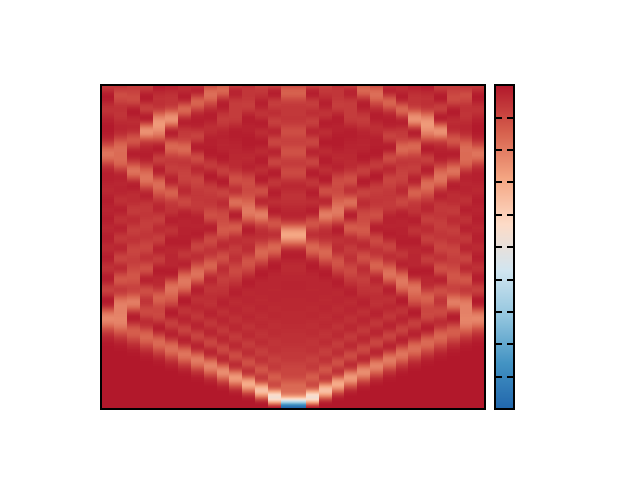
\includegraphics{Sz2_l0_mu0_1}}%
    \gplfronttext
  \end{picture}%
\endgroup
